\section{Neural kinematic basis comparison}
\label{app:nkb}
We compare the learned spectral spans with a direct-velocity neural kinematic basis (NKB), following the camera-ready formulation of \citet{liu2025neural}. Each NKB model is trained independently at the reported capacity on the original case geometry. Its initial coefficients are obtained from the same physical initial velocity through a full-mass least-squares projection. The trajectory comparisons evolve all coordinates autonomously; subsequent reference snapshots are used only for assessment.

\paragraph{Architecture and optimization.}
Our native-CuPy reimplementation uses seven hidden layers of width 256 with LeakyReLU slope $0.01$, followed by an exponential linear unit (ELU) velocity output; LeakyReLU is the leaky rectified linear unit. It optimizes the six NKB penalties with weights $0.01$, $5$, $100$, $30$, $100$, and $100$ for spatial variation, divergence, orthogonality, boundary alignment, mean length, and small length, respectively. The target mean basis length is $0.37$, and the small-length threshold is $0.05$. We realize the orthogonality penalty as the mean squared off-diagonal entry of the global velocity Gram matrix, a nonnegative implementation of the paper's printed signed sum. Spatial Jacobians and their parameter adjoints are evaluated analytically. The periodic model uses sine/cosine coordinates; bounded domains retain their original implicit surfaces and use a soft boundary band of width $0.05$ times the domain side length. Direct velocity outputs use the stated soft kinematic penalties; Eigenfluid uses differential lifts, spectral objectives, and explicit harmonic coordinates.

Each model receives 2000 Adam updates {\citep{kingma2015adam}}, using 4096 points per update in 2D and 6144 in 3D. The learning rate is $5\times10^{-4}\,0.96^{10(s-1)/2000}$ at update $s$, mapping the original ten-epoch decay over this fixed-case budget. Validation uses 4096 points every 25 updates, including the eight original validation geometries in 3D. The common 2000-update protocol compares fixed-case spatial bases, with autonomous assessment at the trajectory capacities. The original NKB geometry-collection experiment uses one million updates; here its shared network architecture and penalties are trained independently for each reported case.

\paragraph{Common evolution and assessment.}
We use the full velocity mass and all output modes, without mode truncation or ridge regularization. The 3D comparison projects the unchanged $128^3$ NS generator, including its Leray projection and normal penalty, onto the NKB span. The periodic and multi-hole comparisons use the same algebraic curl-form operators and integration schemes as the spectral-basis experiments. NKB controls incompressibility and boundary tangency through its penalties. The common Galerkin assessment measures how this spatial representation supports the same reduced evolution used for the spectral bases. The original NKB solver couples its basis to semi-Lagrangian advection and reprojection.

Periodic errors use the common $128^2$ observation grid and all 241 frames through $T=18\pi$, with vortex separation $d=1.35$. NKB operator quadrature uses $256^2$ points. The multi-hole assessment uses all original common-domain points, the level-2 reference, 20 initial states, and 51 frames to $T=1$. The 3D assessment retains all 1,599,754 fluid nodes and 30 frames to $T=1.16$. Training, offline assembly, and online integration are separate costs. \docref{Table}{tab:nkb-matched} gives the 2D initial projection errors, \docref{Figure}{fig:nkb-completed} compares autonomous errors with same-capacity controls, and \docref{Table}{tab:runtime-training} records training costs.

\begin{table}[!htb]
\centering\small
\caption{Initial full-mass projection errors for the 2D NKB adaptation at $K=1024$ (\%). Periodic entries are mean $\pm$ sample SD over three seeds; multi-hole entries average 20 initial states. Trajectory comparisons are shown in \docref{Figure}{fig:nkb-completed}, 3D initial errors in \docref{Figure}{fig:case3-capacity}(b), and NKB training costs in \docref{Table}{tab:runtime-nkb-training}.}
\label{tab:nkb-matched}
\begin{tabular}{lr}\toprule
Case&Initial velocity error (\%)\\\midrule
Periodic &$2.493\pm0.138$\\
One hole&20.760\\
Two holes&22.566\\
Three holes&22.201\\
\bottomrule\end{tabular}
\end{table}

\paragraph{Kinematic residuals and numerical refinement.}
The periodic NKB initial states have a three-seed mean divergence-to-curl norm ratio of $0.195$. Their full-mass condition numbers range from $1.236\times10^{8}$ to $1.899\times10^{8}$. The maximum double-time-step trajectory difference is $4.412\times10^{-12}$. For seed 0, the $128^2$ to $256^2$ operator-quadrature trajectory sensitivity on this same case is $46.100\%$; these measurements separately characterize spatial quadrature and temporal resolution.

For the one-, two-, and three-hole domains, respectively, the mean initial divergence-to-curl ratios are $(0.721,0.770,0.722)$ and the sampled boundary-normal root mean square (RMS) relative to domain velocity RMS is $(0.170,0.216,0.231)$. Maximum trajectory differences under time-step refinement are $(7.03\times10^{-6},1.26\times10^{-5},4.15\times10^{-6})$; those under operator-quadrature refinement are $(1.24\times10^{-2},3.94\times10^{-3},2.99\times10^{-3})$.

\paragraph{Three-dimensional trajectory and kinematic diagnostics.}
\docref{Tables}{tab:nkb-3d-checks} and~\ref{tab:nkb-3d-kinematics} supplement the final errors with trajectory means, full-mass conditioning, and initial/final kinematic residuals. The trajectory mean averages all 30 stored frames, including $t=0$ and $T=1.16$. The mass condition number $\kappa(M)$ is the largest-to-smallest eigenvalue ratio of the symmetric FP64 mass matrix; all $K$ coordinates are retained.

\begin{table}[!htb]
\centering\small
\caption{Completed 3D NKB trajectories and numerical checks. Mean error is relative velocity $L^2$ in percent. Right-hand-side (RHS) discrepancy compares the assembled coefficient RHS with the projected full-grid RHS at $0.2c_0$ and $c_0$, taking the larger relative Euclidean error. The final column is the maximum relative mass-norm trajectory difference between $\Delta t=0.00125$ and $0.000625$. These checks measure operator agreement and time-step sensitivity on the fixed $128^3$ grid.}
\label{tab:nkb-3d-checks}
\begin{tabular}{rrrrr}\toprule
$K$&Mean error (\%)&$\kappa(M)$&RHS discrepancy&Time-step difference\\\midrule
128&90.170&$5.51\times10^{5}$&$2.37\times10^{-10}$&$9.39\times10^{-12}$\\
256&85.572&$5.58\times10^{6}$&$2.04\times10^{-9}$&$2.14\times10^{-11}$\\
512&78.442&$1.17\times10^{8}$&$5.33\times10^{-8}$&$3.86\times10^{-11}$\\
1024&66.826&$4.33\times10^{9}$&$9.92\times10^{-8}$&$5.00\times10^{-11}$\\
\bottomrule\end{tabular}
\end{table}

For the grid-reconstructed velocity (zero in solid cells), let $\mathbf k$ be the grid Fourier wavevector and $\widehat u$ its Fourier transform, with $\|\cdot\|_2$ the Euclidean norm over Fourier samples. Let $\langle\cdot\rangle_{\mathcal B}$ denote the mean over the original boundary band $\mathcal B$, and $\mathcal P_h$ the original grid Leray projection with componentwise dealiasing and the zero-mean constraint. The divergence ratio $D$, boundary-normal ratio $B$, and grid-correction ratio $P$ are
\begin{align*}
D&=\frac{\|i\mathbf k\cdot\widehat u\|_2}{\||\mathbf k|\widehat u\|_2},&
B&=\left(\frac{\langle(u\cdot n)^2\rangle_{\mathcal B}}{\langle|u|^2\rangle_{\mathcal B}}\right)^{1/2},&
P&=\frac{\|\mathcal P_hu-u\|_2}{\|u\|_2}.
\end{align*}
Here $D$ uses the full velocity-gradient norm, whereas the 2D diagnostic uses the curl norm; $B$ is a band-sampled RMS ratio.

\begin{table}[!htb]
\centering\small
\caption{Initial and final 3D NKB kinematic residuals on the original $128^3$ grid. All entries are dimensionless ratios, using the definitions above.}
\label{tab:nkb-3d-kinematics}
\begin{tabular}{rrrrrrr}\toprule
&\multicolumn{2}{c}{Divergence $D$}&\multicolumn{2}{c}{Boundary normal $B$}&\multicolumn{2}{c}{Grid correction $P$}\\
\cmidrule(lr){2-3}\cmidrule(lr){4-5}\cmidrule(lr){6-7}
$K$&Initial&Final&Initial&Final&Initial&Final\\\midrule
128&0.447&0.328&0.395&0.212&0.401&0.312\\
256&0.472&0.385&0.431&0.272&0.373&0.519\\
512&0.430&0.391&0.368&0.222&0.304&0.470\\
1024&0.364&0.385&0.271&0.175&0.224&0.435\\
\bottomrule\end{tabular}
\end{table}




\begin{figure}[!htb]
\centering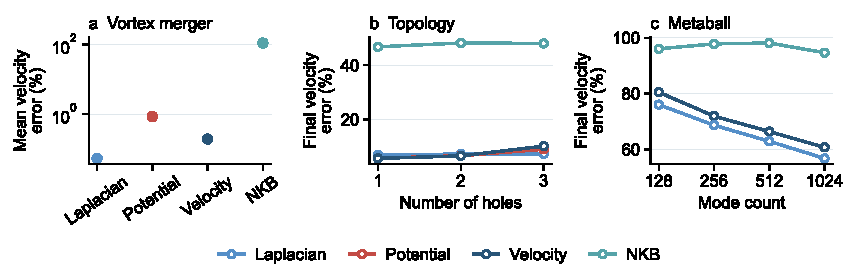
\includegraphics[width=\linewidth,height=.72\textheight,keepaspectratio]{unified_names_20261021_v1/nkb_completed_comparison.pdf}
\caption{\textbf{NKB and Eigenfluid under matched case assessment.} (a) Vortex-merger mean trajectory error over 241 frames, $K=1024$, three learned seeds with one sample SD. (b) Final errors for the three topologies, averaged over 20 states. (c) Metaball capacity comparison against the same original reference. NKB uses the stated 2000-update, common-Galerkin adaptation. Numerical denotes the same-capacity Laplacian control.}
\label{fig:nkb-completed}
\end{figure}
